\documentclass[rodrigo]{wtpc-beamer}
% Las opciones posibles para autores son:
% cecilia, graciela, pablo, rodrigo

% Aquí va el título. Nuestra información (nombre, mail, color de cada
% uno) está en wtpc-beamer.cls.
\title[Ejemplos con wtpc-beamer.cls]{Lista de ejemplos para la utilización de wtpc-beamer.cls}


%%%%%%%%%%%%%%%%%%%%%%%%%%%%%%%%%%%%%%%%%%%%%%%%%%%%%%%%%%%%%%%%%%%%
%%%%%%%%%% DOCUMENT
%%%%%%%%%%%%%%%%%%%%%%%%%%%%%%%%%%%%%%%%%%%%%%%%%%%%%%%%%%%%%%%%%%%%
\begin{document}

% This frame is the title frame
\frame{\titlepage}


% En principio, las secciones no tienen razón de ser, pero podrían ser útiles.
\section{Introduction}
\frame{\frametitle{Ejemplos para utilizar la clase wtpc.cls}

  Por ahora, no hay demasiadas cosas raras para la utilización de esta
  clase de Beamer. Se utiliza como se utiliza Beamer, pero está
  simplificado el asunto de poner código. Además, la paleta de colores
  con la que se muestra el código es fácilmente modificable (por si no
  nos gusta o se ve mal en algún proyector).

  Pasemos a ver unos ejemplos.
}

\frame{\frametitle{Incluir código desde un archivo}
  Para incluir código desde un archivo, utilizamos el paquete
  lstlistings. Si bien hay otros (minted, por ejemplo), este paquete
  es el más portable, ya que no requiere programas adicionales
  instalados en el sistema (minted, por ejemplo, requiere instalar
  pygmentize).

  Entonces, para incluir código de, por ejemplo, C, ponemos:
  \includecode{style=C}{code/code_ex.c}
}

\frame{\frametitle{Incluir código desde un archivo}
  O si queremos incluir algo del $shell$, directamente:
  \includeshell{code/code_ex.sh}
}

\frame{\frametitle{Incluir código \textit{inline}}

  Si queremos introducir algo de código \textit{inline}, es tan
  sencillo como poner \codeinline{Python}{import numpy as np} en el
  caso de código propiamente dicho, o \shellinline{for i in
    $(ls); do echo $i; done} para comandos de la consola.
}


\begin{frame}[fragile]\frametitle{Incluir código desde \LaTeX}
  
  Si queremos incluir código desde \LaTeX, es un poco más
  complicado. Hacerlo, requiere que la diapositiva (frame) sea
  iniciada con la opción [fragile] (hay un 'conflicto' con entorno
  verbatim, necesario para que \LaTeX~no intente interpretar en código
  que le estamos poniendo). De cualquier forma, si iniciamos la
  diapositiva con \textbackslash begin\{frame\}[fragile] (y la
  cerramos con \textbackslash end\{frame\}), todo anda bien.
\end{frame}

\begin{frame}[fragile]\frametitle{Incluir código desde \LaTeX}
  Hecho esto, podemos incluir el código de la siguiente manera:
\begin{code}{style=Python}
import numpy as np
class prueba(object):
  def __init__(self, var1):
  """clase prueba"""
  self.variable = var1
\end{code}
\end{frame}

\begin{frame}[fragile]\frametitle{Incluir código desde \LaTeX}
  Cabe mencionar que si agregamos código así, tengamos cuidado, porque
  los espacios en blanco que escribamos los va a considerar. Por
  ejemplo, vean qué sucede si sigo la \textit{indentación} que vengo
  usando en \LaTeX:
  \begin{code}{style=Python}
    import numpy as np
    class prueba(object):
      def __init__(self, var1):
      """clase prueba"""
      self.variable = var1
  \end{code}
  Noten no sólo que la \textit{indentación} es más grande, sino también que los dos espacios antes de \textbackslash end\{code\} los tomó como una línea de código extra.

  Conclusión: en general es más cómodo usar \textbackslash includecode (o \textbackslash includeshell).
\end{frame}

\begin{frame}[fragile]\frametitle{Incluir código desde \LaTeX}
  Para agregar una consola:
\begin{shell}
#!/bin/sh
echo ``Hello world''
\end{shell}
\end{frame}

\frame{\frametitle{Cosas copadas de lstlisting}
  Hay algunas opciones de lstlisting que nos pueden venir bien.
  \begin{itemize}
    \item Poner determinadas líneas del código:
      \includecode{style=C,firstline=1,lastline=3}{code/code_ex.c}
    \item La magnífica posibilidad de resaltar líneas:
      \includecode{style=Python, linebackgroundcolor={%
    \btLstHL<1>{1-3}% on slide 1, highlight lines 1-3
    \btLstHL<2>{4}% on slide 2, highlight lines 6 and 9
    \btLstHL<3>{5}%
  }}{code/code_ex.py}

  \end{itemize}
}

\frame{\frametitle{Incluir figuras, etc}
  Para la inclusión de figuras, se sigue la misma lógica de
  siempre. Puede ser incluida con el entorno \textit{figure}:
  \begin{figure}
    \centering
    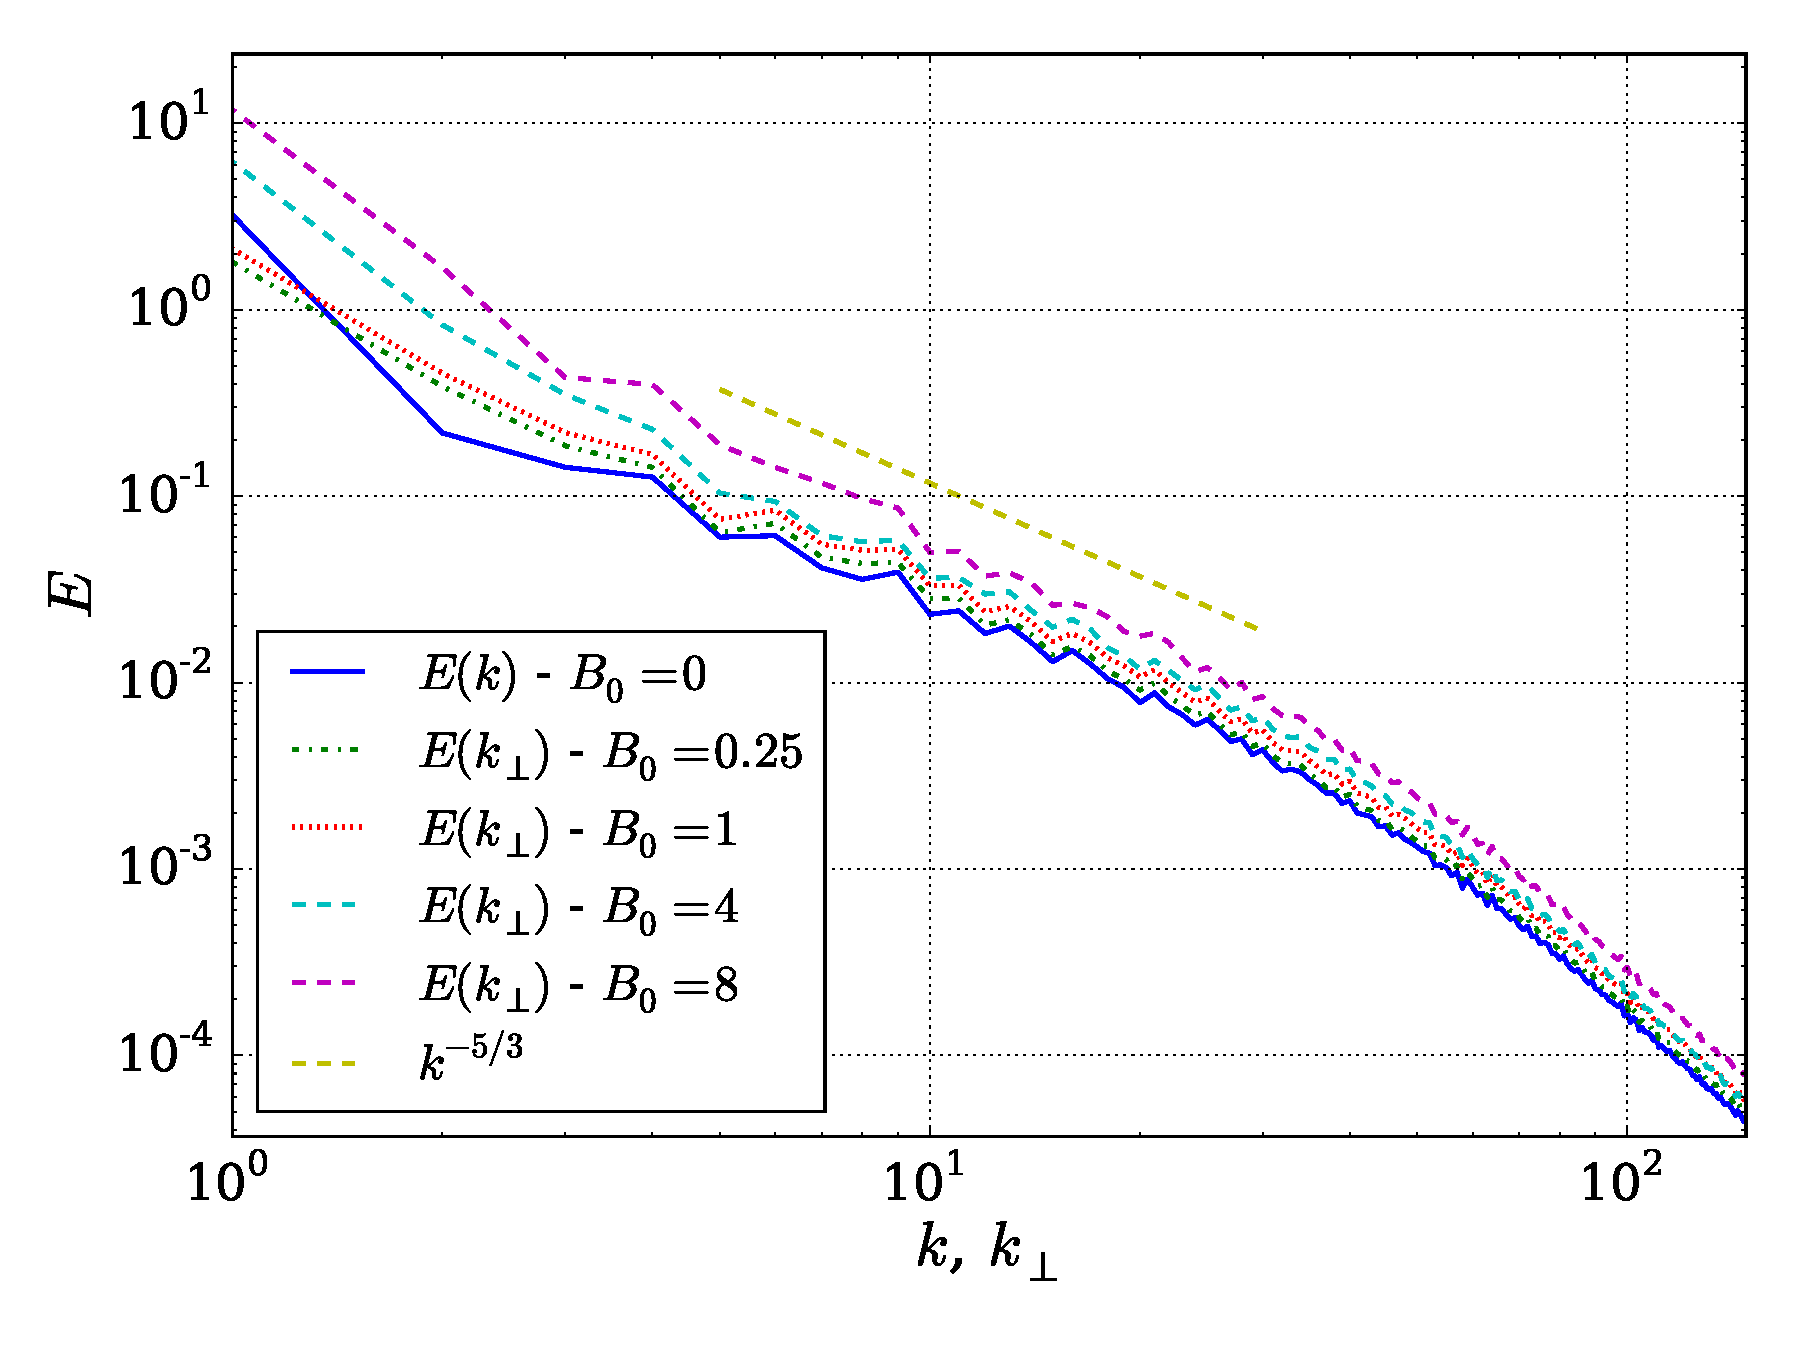
\includegraphics[width=0.5\columnwidth]{figs/fig1_E.pdf}
    \caption{Reduced perpendicular energy spectra $E(k_\perp)$ for the
      simulations with $B_0=0.25$, $1$, $4$, and $8$, and isotropic energy
      spectrum $E(k)$ for the simulation with $B_0=0$. Kolmogorov
      scaling, $\sim k_\perp^{-5/3}$, is shown as reference.}
    \label{fig1:E}
  \end{figure}
}

\frame{\frametitle{Incluir figuras, etc}
  O con entorno \textit{subfigure}:
  
  \begin{figure}
    \centering
          
    \subfigure[$k_\parallel = 0$]{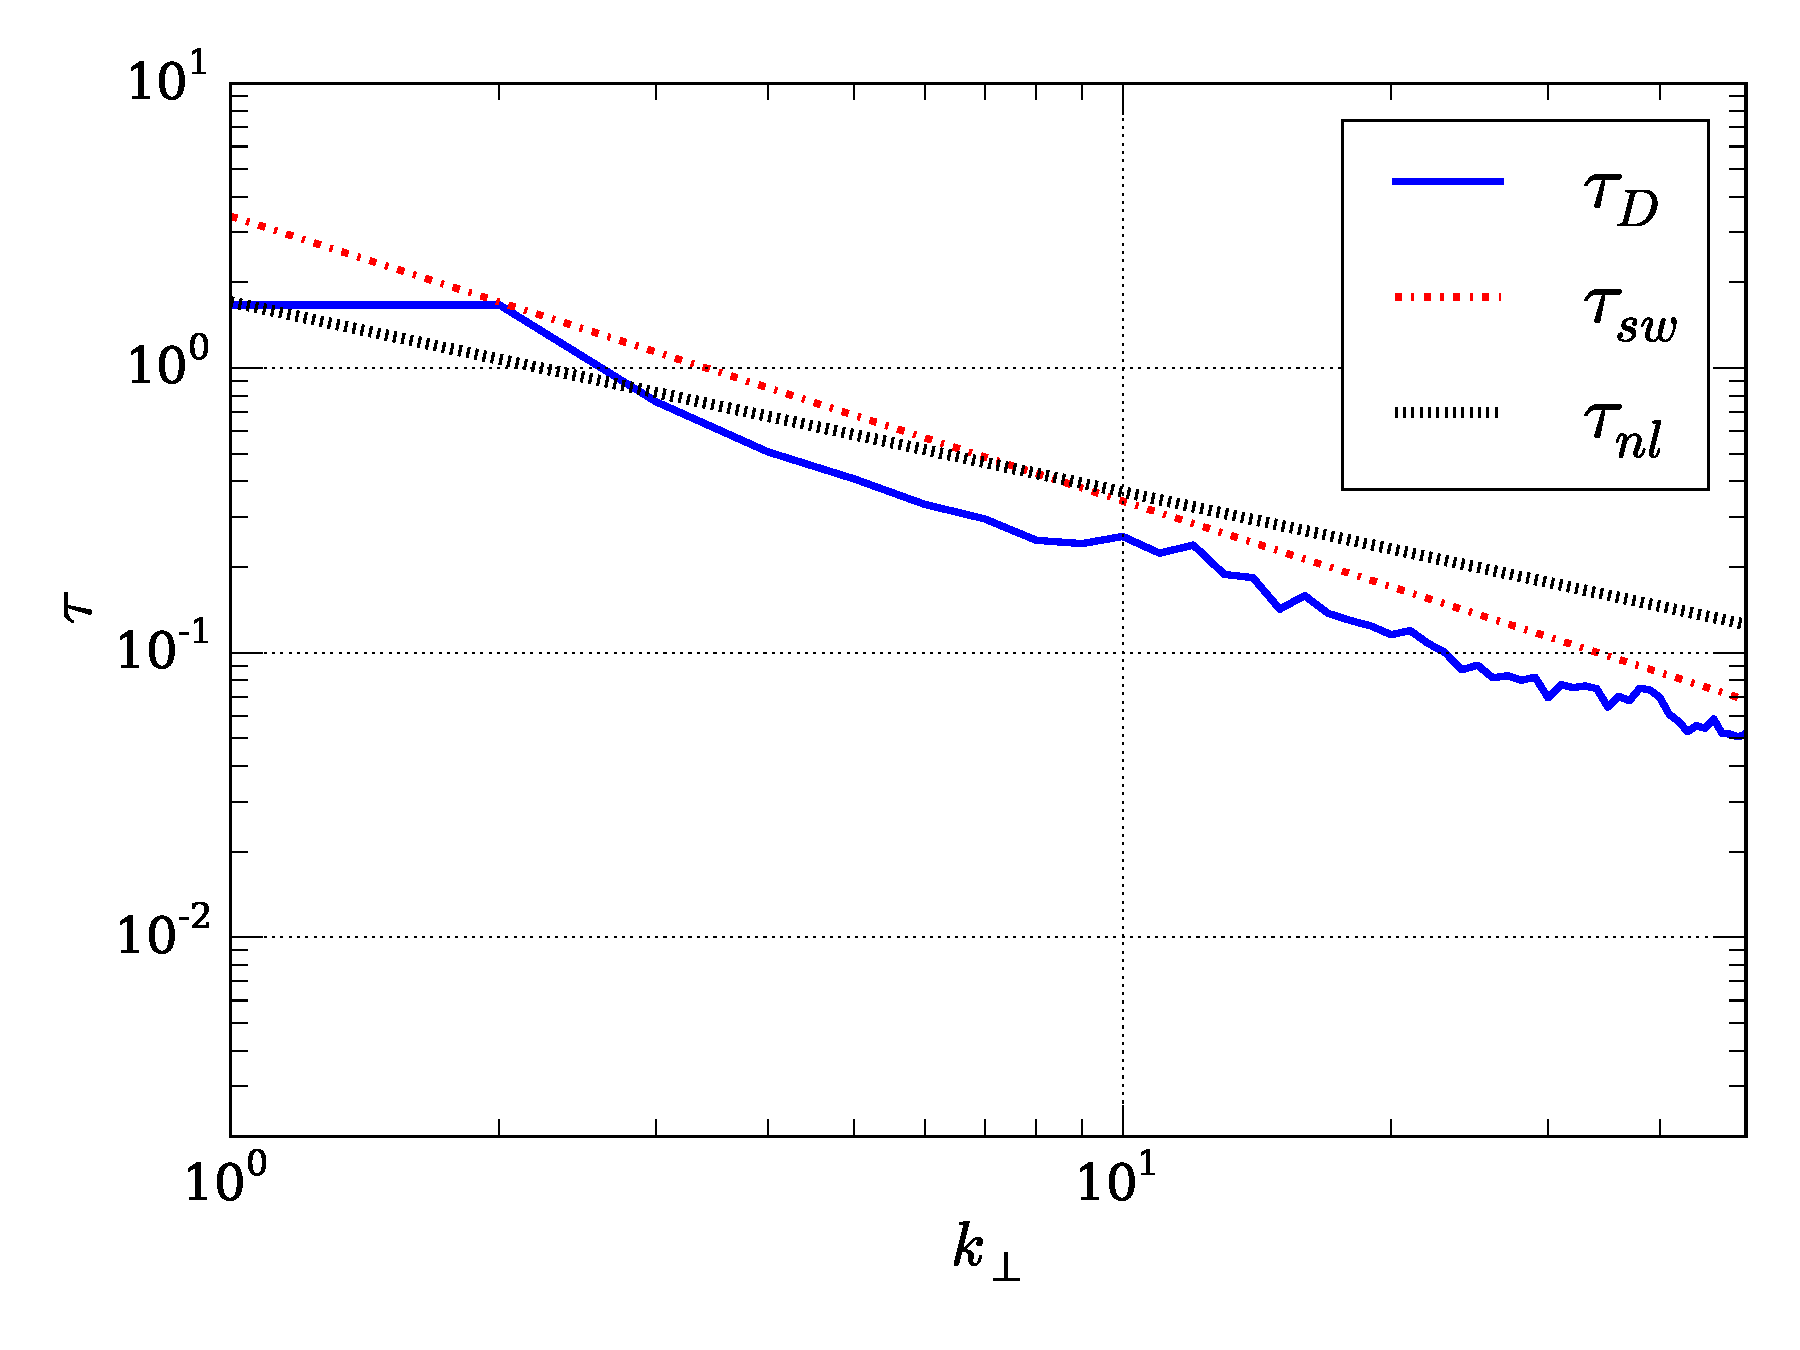
\includegraphics[width=0.3\columnwidth]{figs/fig5_B8_b_kpara_0.pdf}}
    \subfigure[$k_\parallel = 10$]{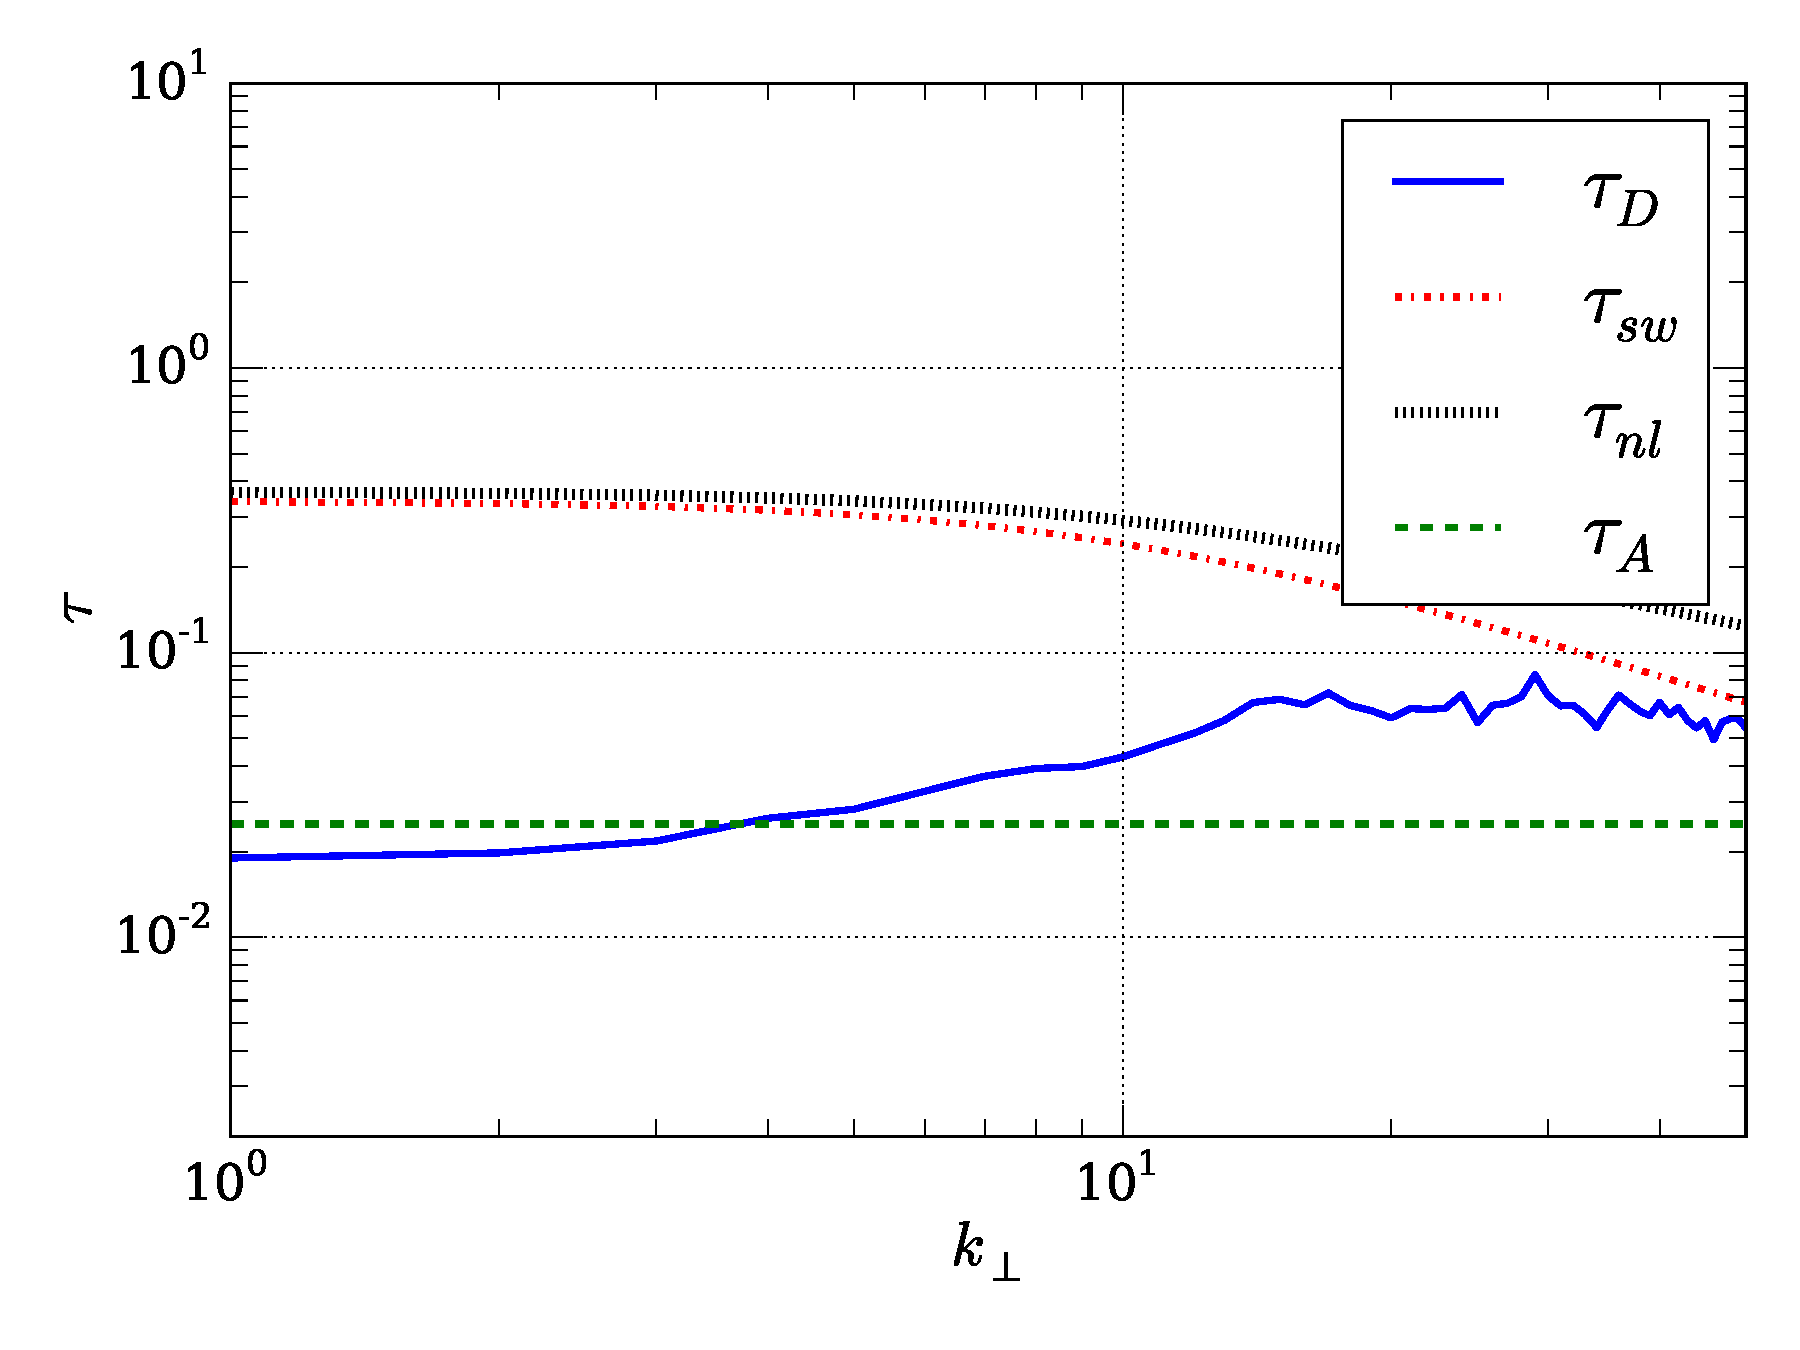
\includegraphics[width=0.3\columnwidth]{figs/fig5_B8_b_kpara_10.pdf}}

    \subfigure[$k_\parallel = 20$]{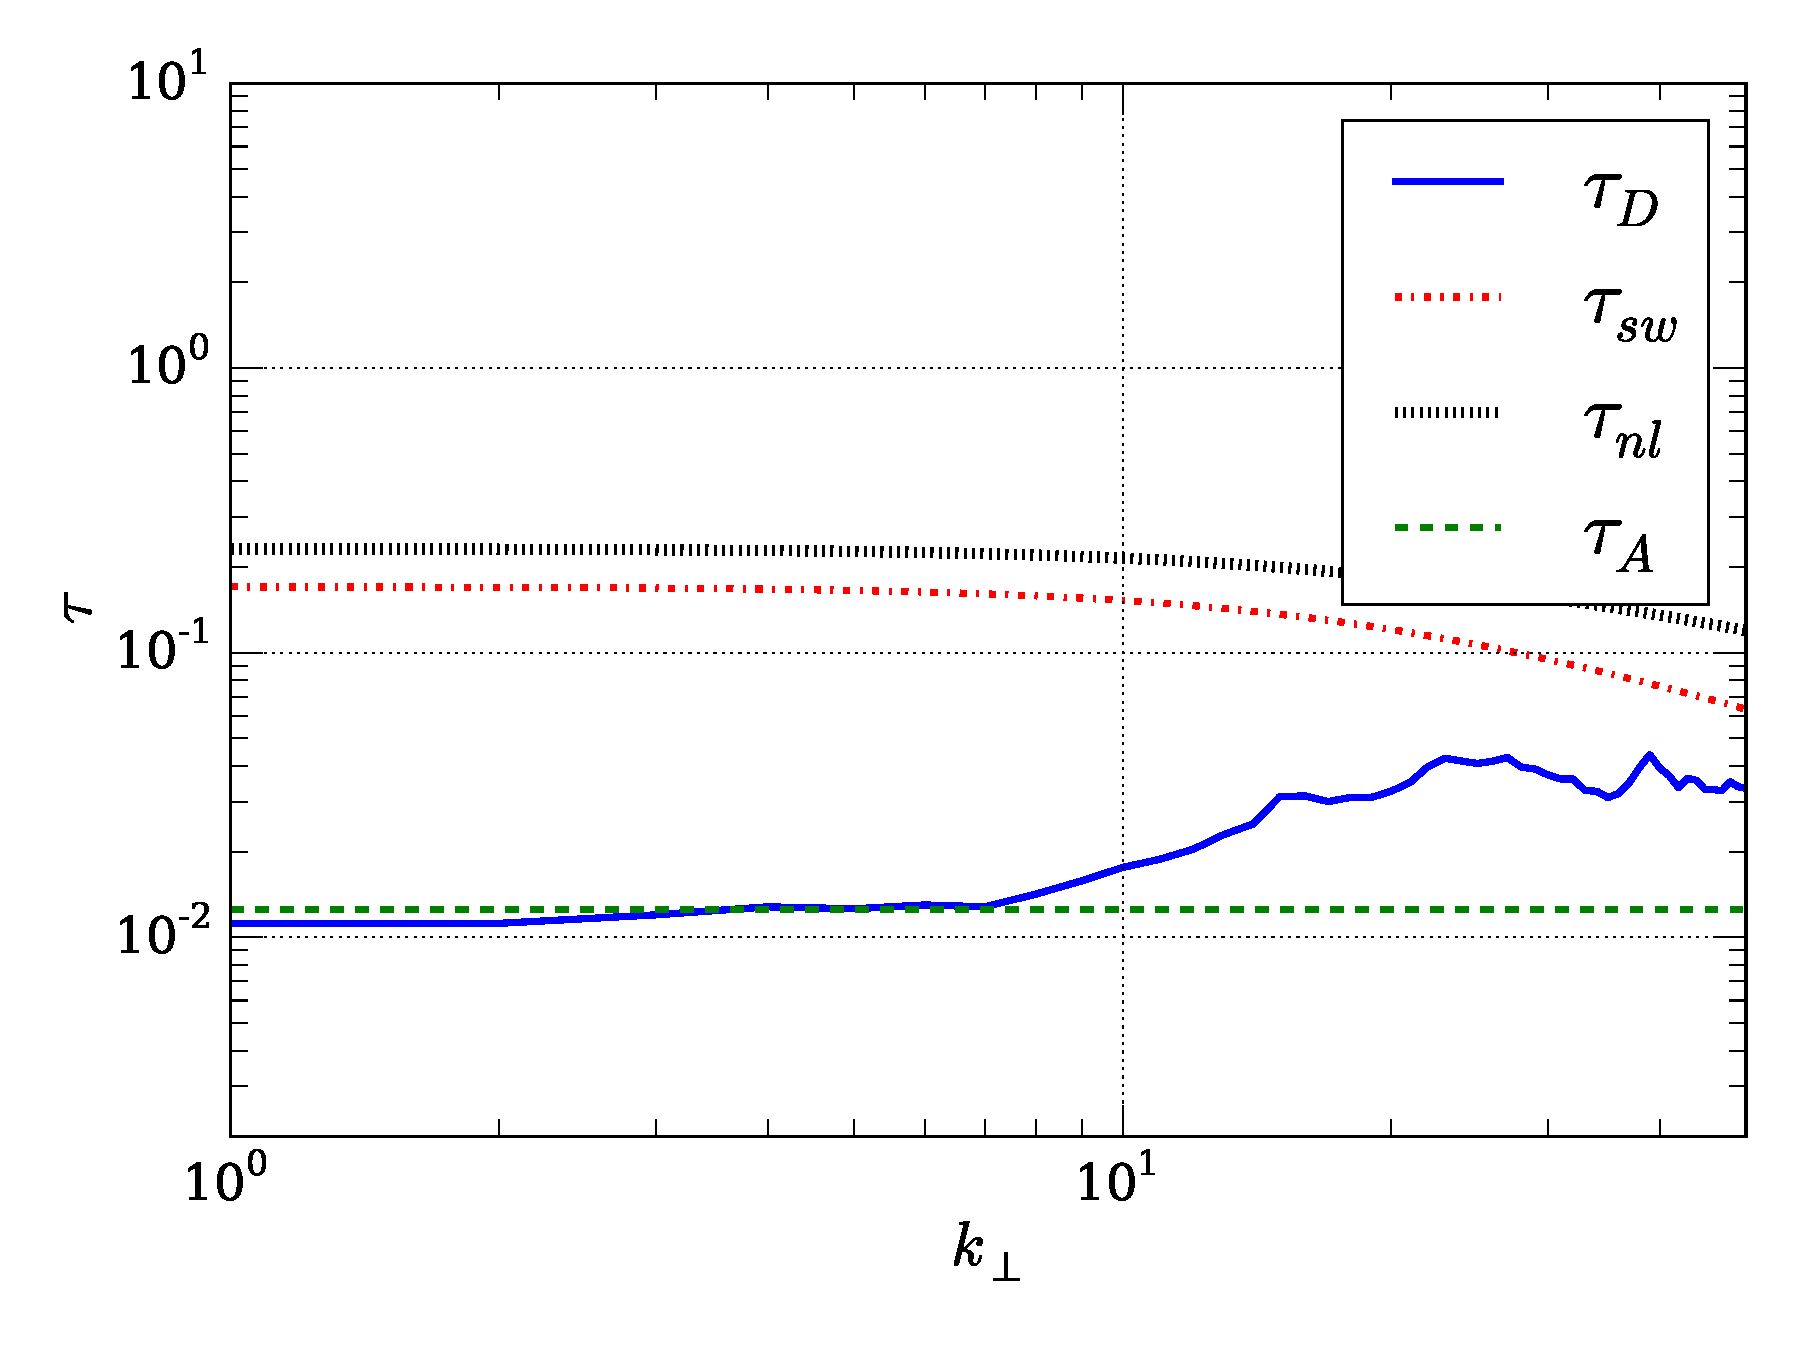
\includegraphics[width=0.3\columnwidth]{figs/fig5_B8_b_kpara_20.pdf}}
    \caption{Correlation functions
      $\Gamma(k_\perp=0,k_\parallel=k_0,\tau)$ and
      $\Gamma(k_\perp=k_0,k_\parallel=0,\tau)$ as a function of the lag
      time $\tau$, for $k_0=5$, 10, 15, and 20, in the simulation with
      $B_0=1$. The value of $\tau$ for which $\Gamma=1/e$ (horizontal
      dotted line) corresponds to the decorrelation time $\tau_D$ for
      each value of $\vec{k}$.}
    \label{subfigs}
  \end{figure}
}


\frame{\frametitle{Incluir figuras, etc}
  También lo podemos incluir más a arcaicamente:
  \begin{center}
    $k_\parallel = 20$\\
    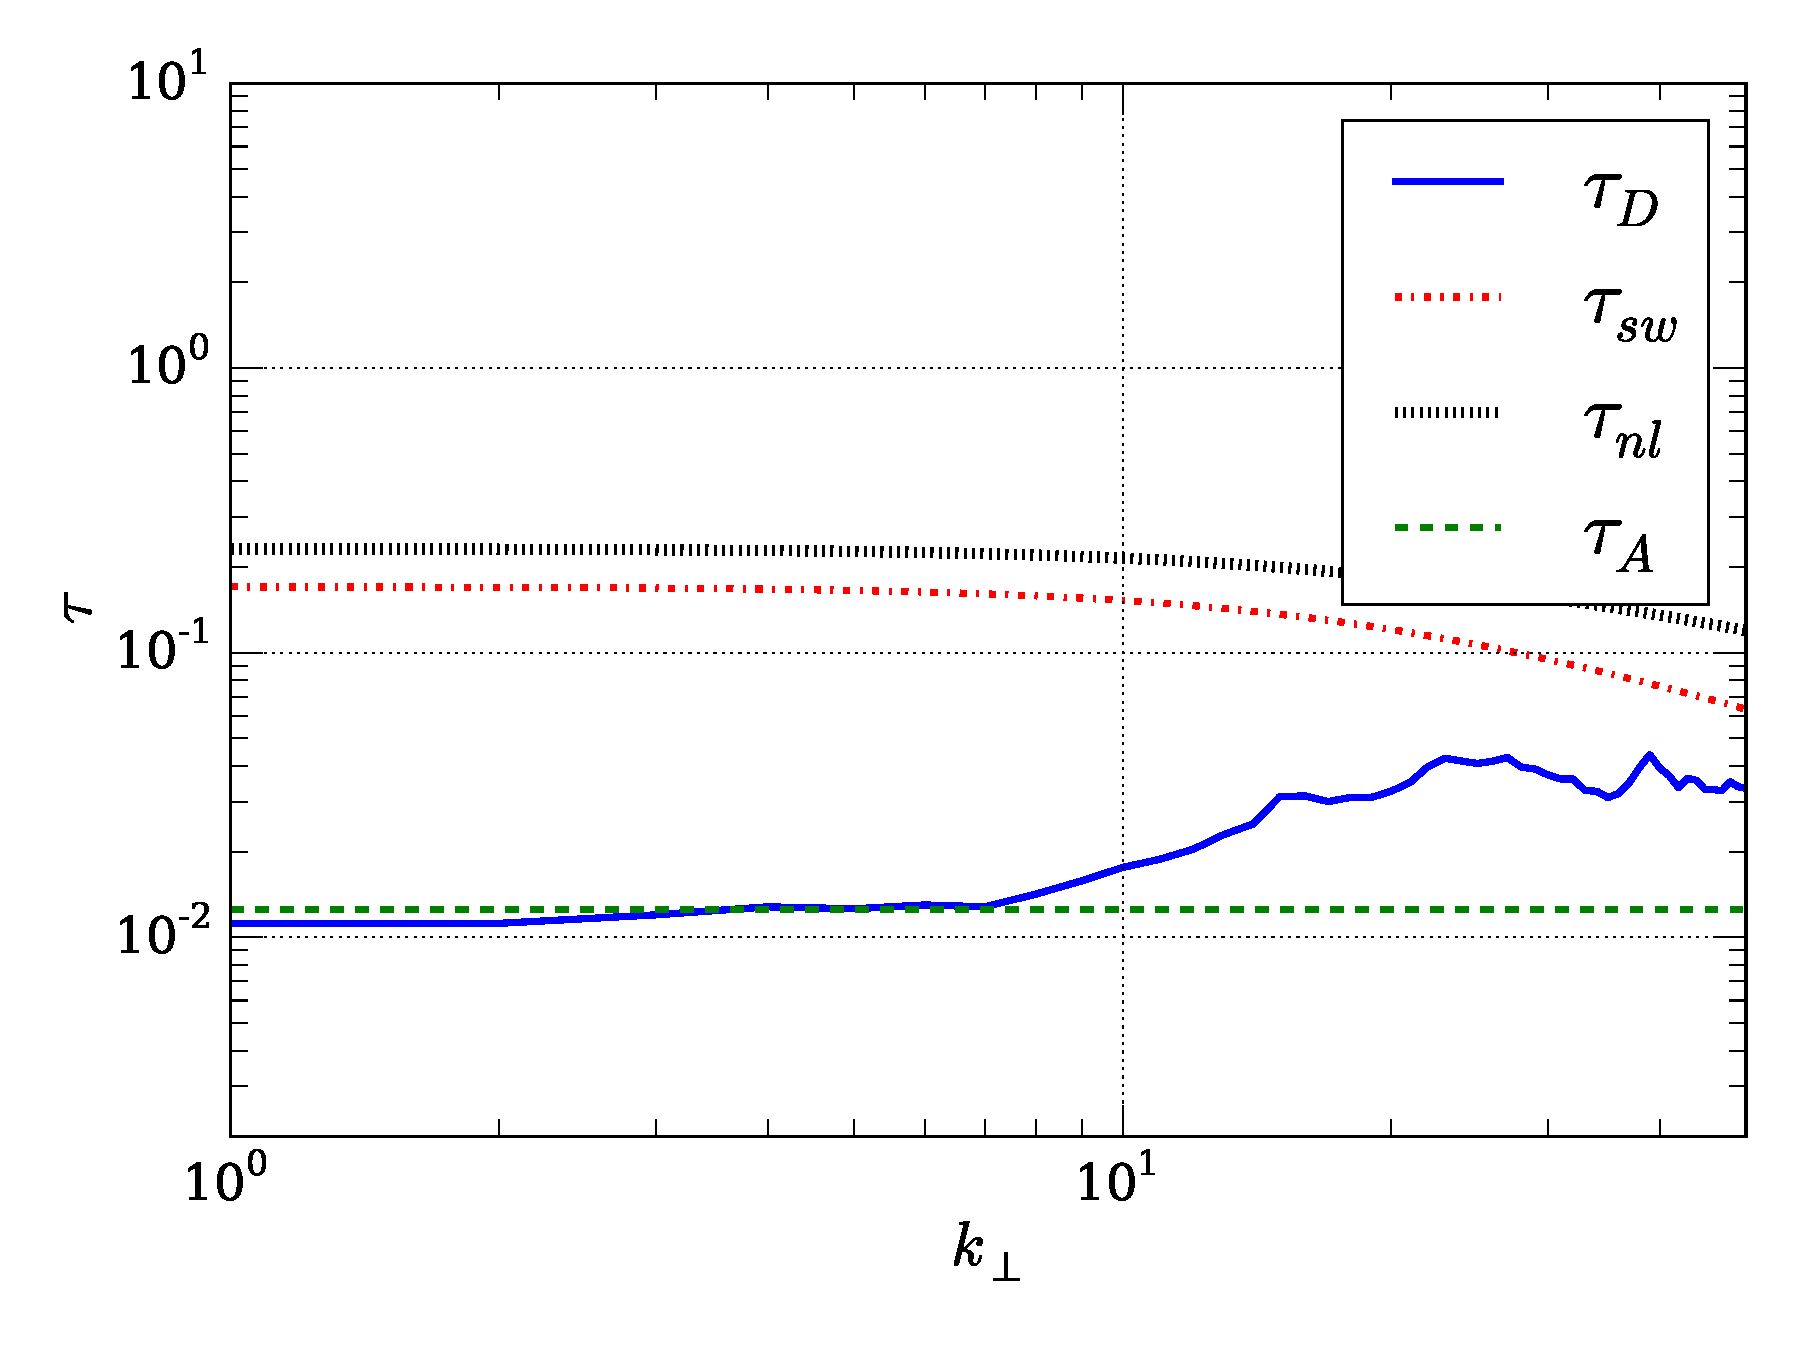
\includegraphics[width=0.38\columnwidth]{figs/fig5_B8_b_kpara_20.pdf} \\
  \end{center}
}

\frame{\frametitle{Incluir figuras, etc}
  Y es posible que necesitemos utilizar \textit{minipage}s:

  \centering  
  \begin{minipage}[t]{0.49\textwidth}
    \begin{center}
      $k_\parallel = 0$\\
      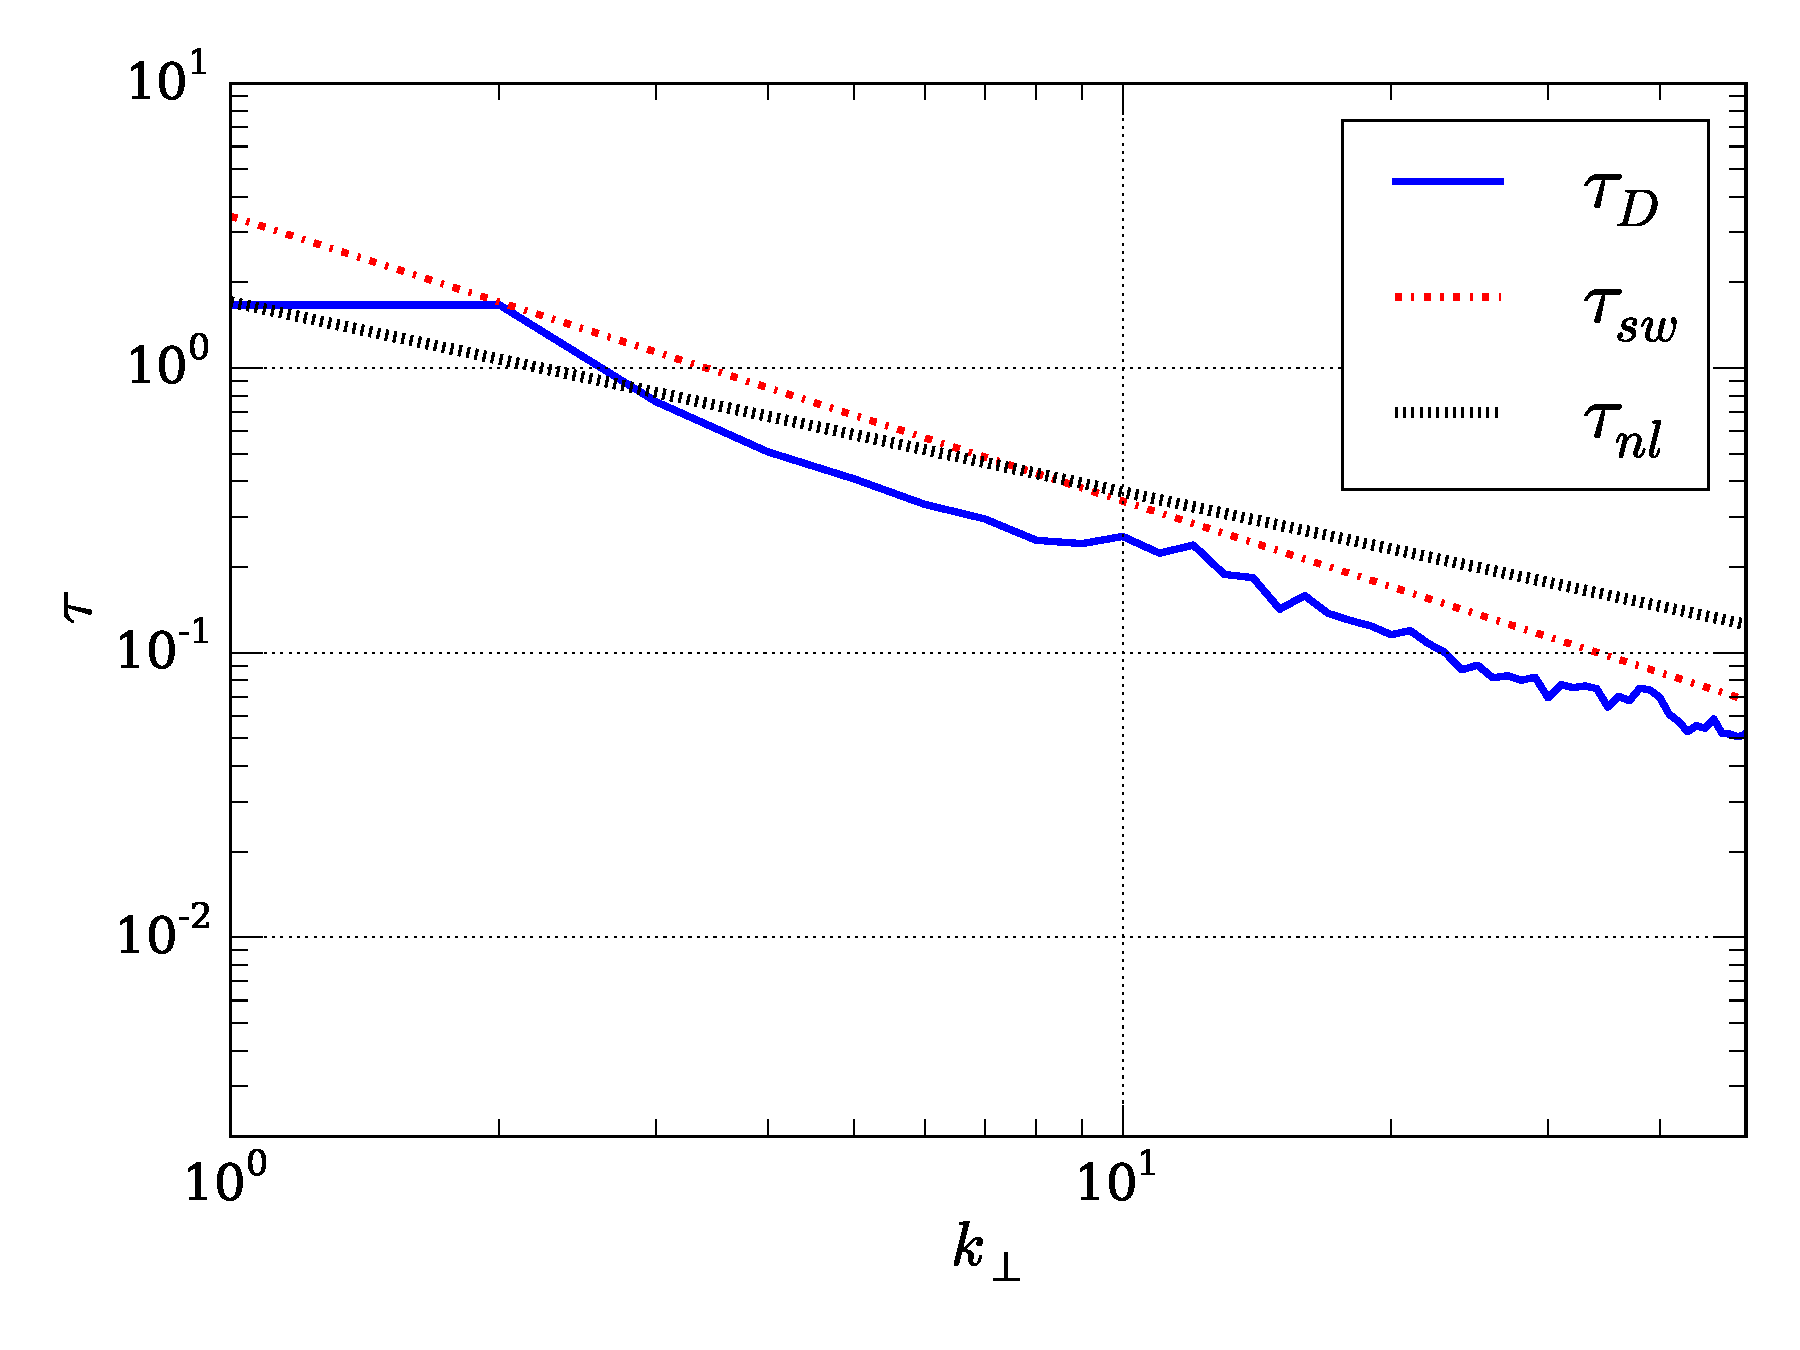
\includegraphics[width=0.7\columnwidth]{figs/fig5_B8_b_kpara_0.pdf}
    \end{center}
  \end{minipage}
  \begin{minipage}[t]{0.49\textwidth}
    \begin{center}
      $k_\parallel = 10$\\
      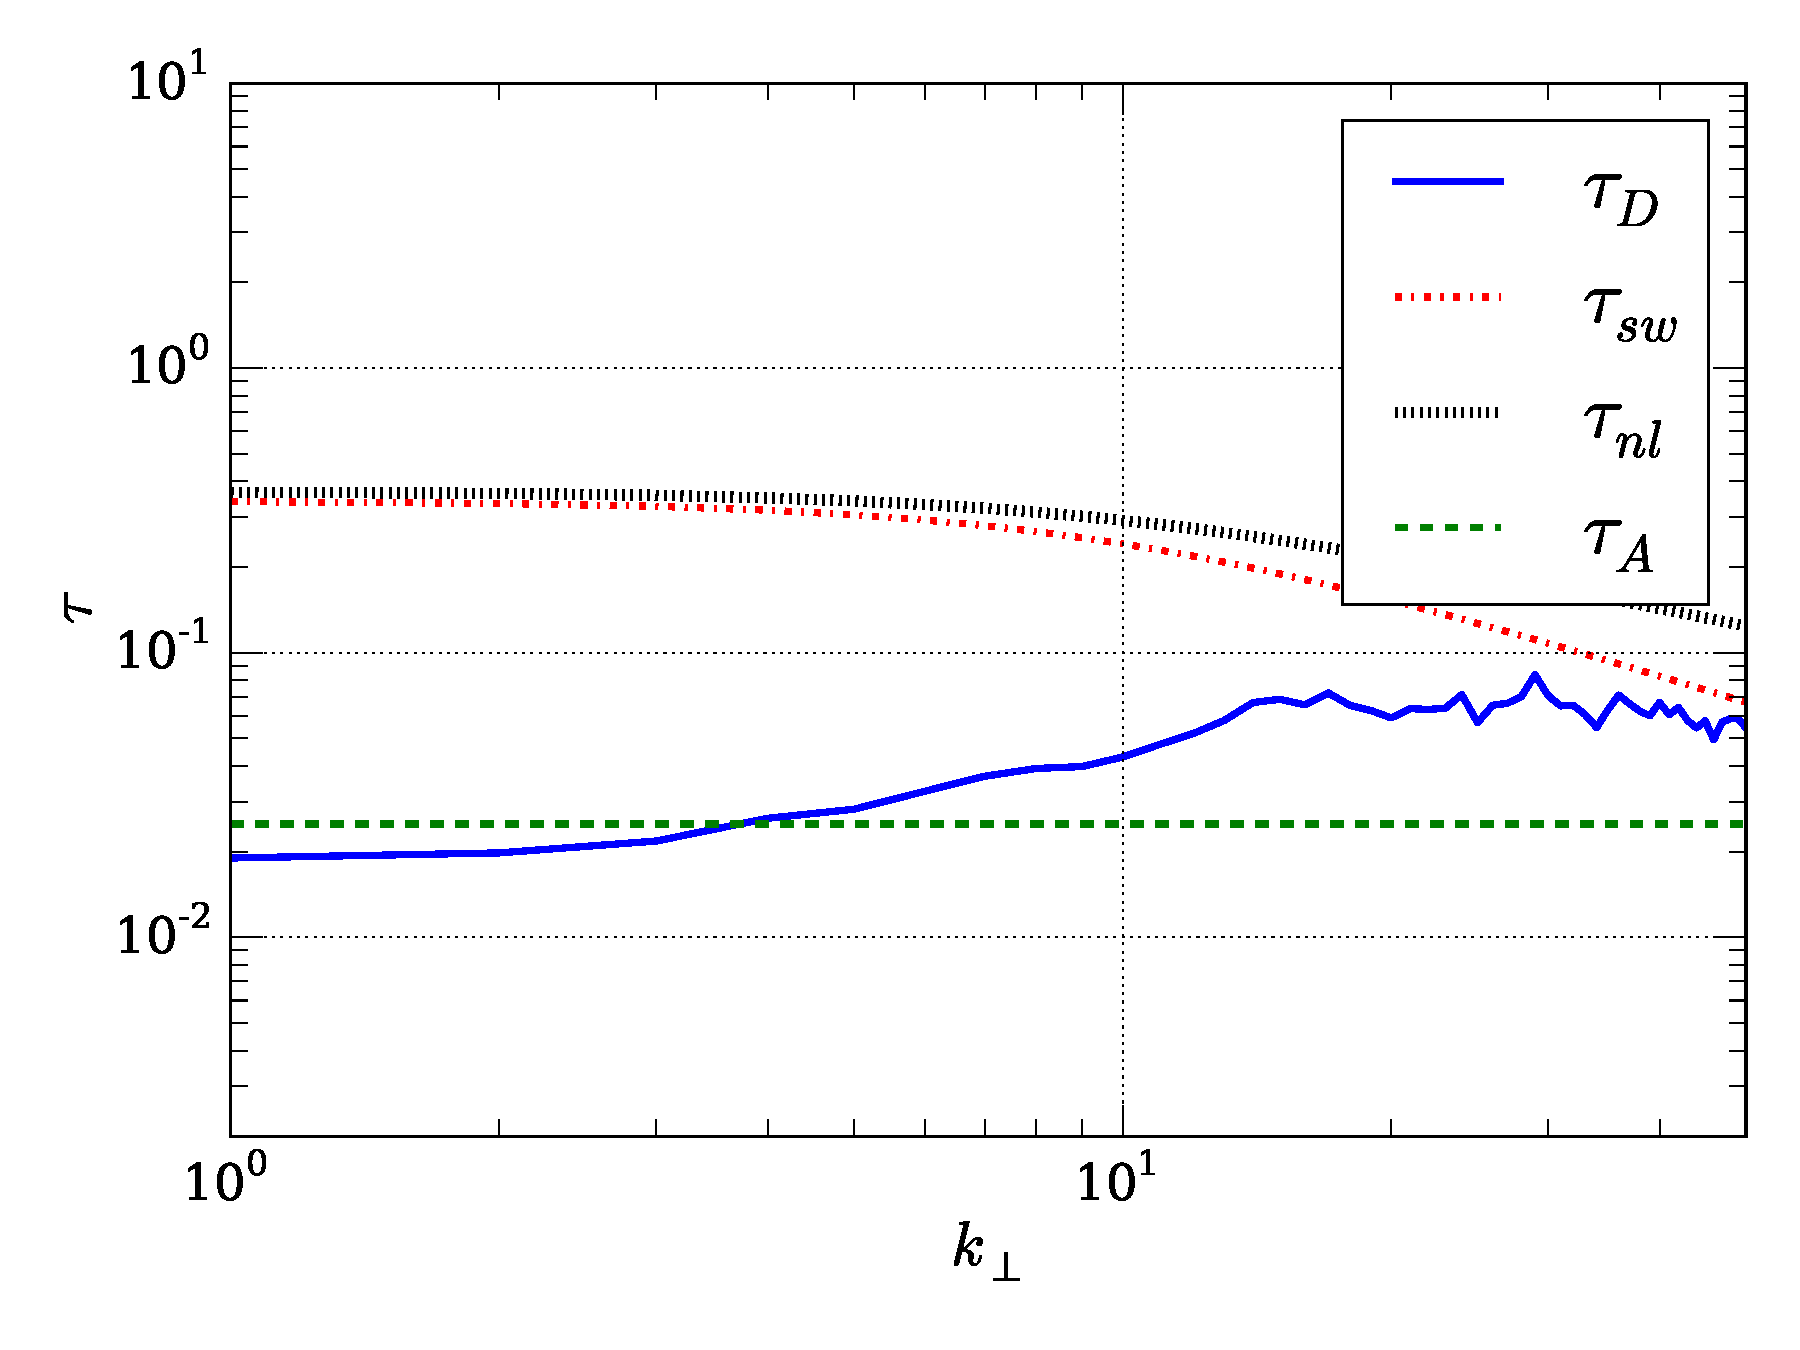
\includegraphics[width=0.7\columnwidth]{figs/fig5_B8_b_kpara_10.pdf}
    \end{center}
  \end{minipage}
  \begin{minipage}[t]{0.49\textwidth}
    \begin{center}
      $k_\parallel = 20$\\
      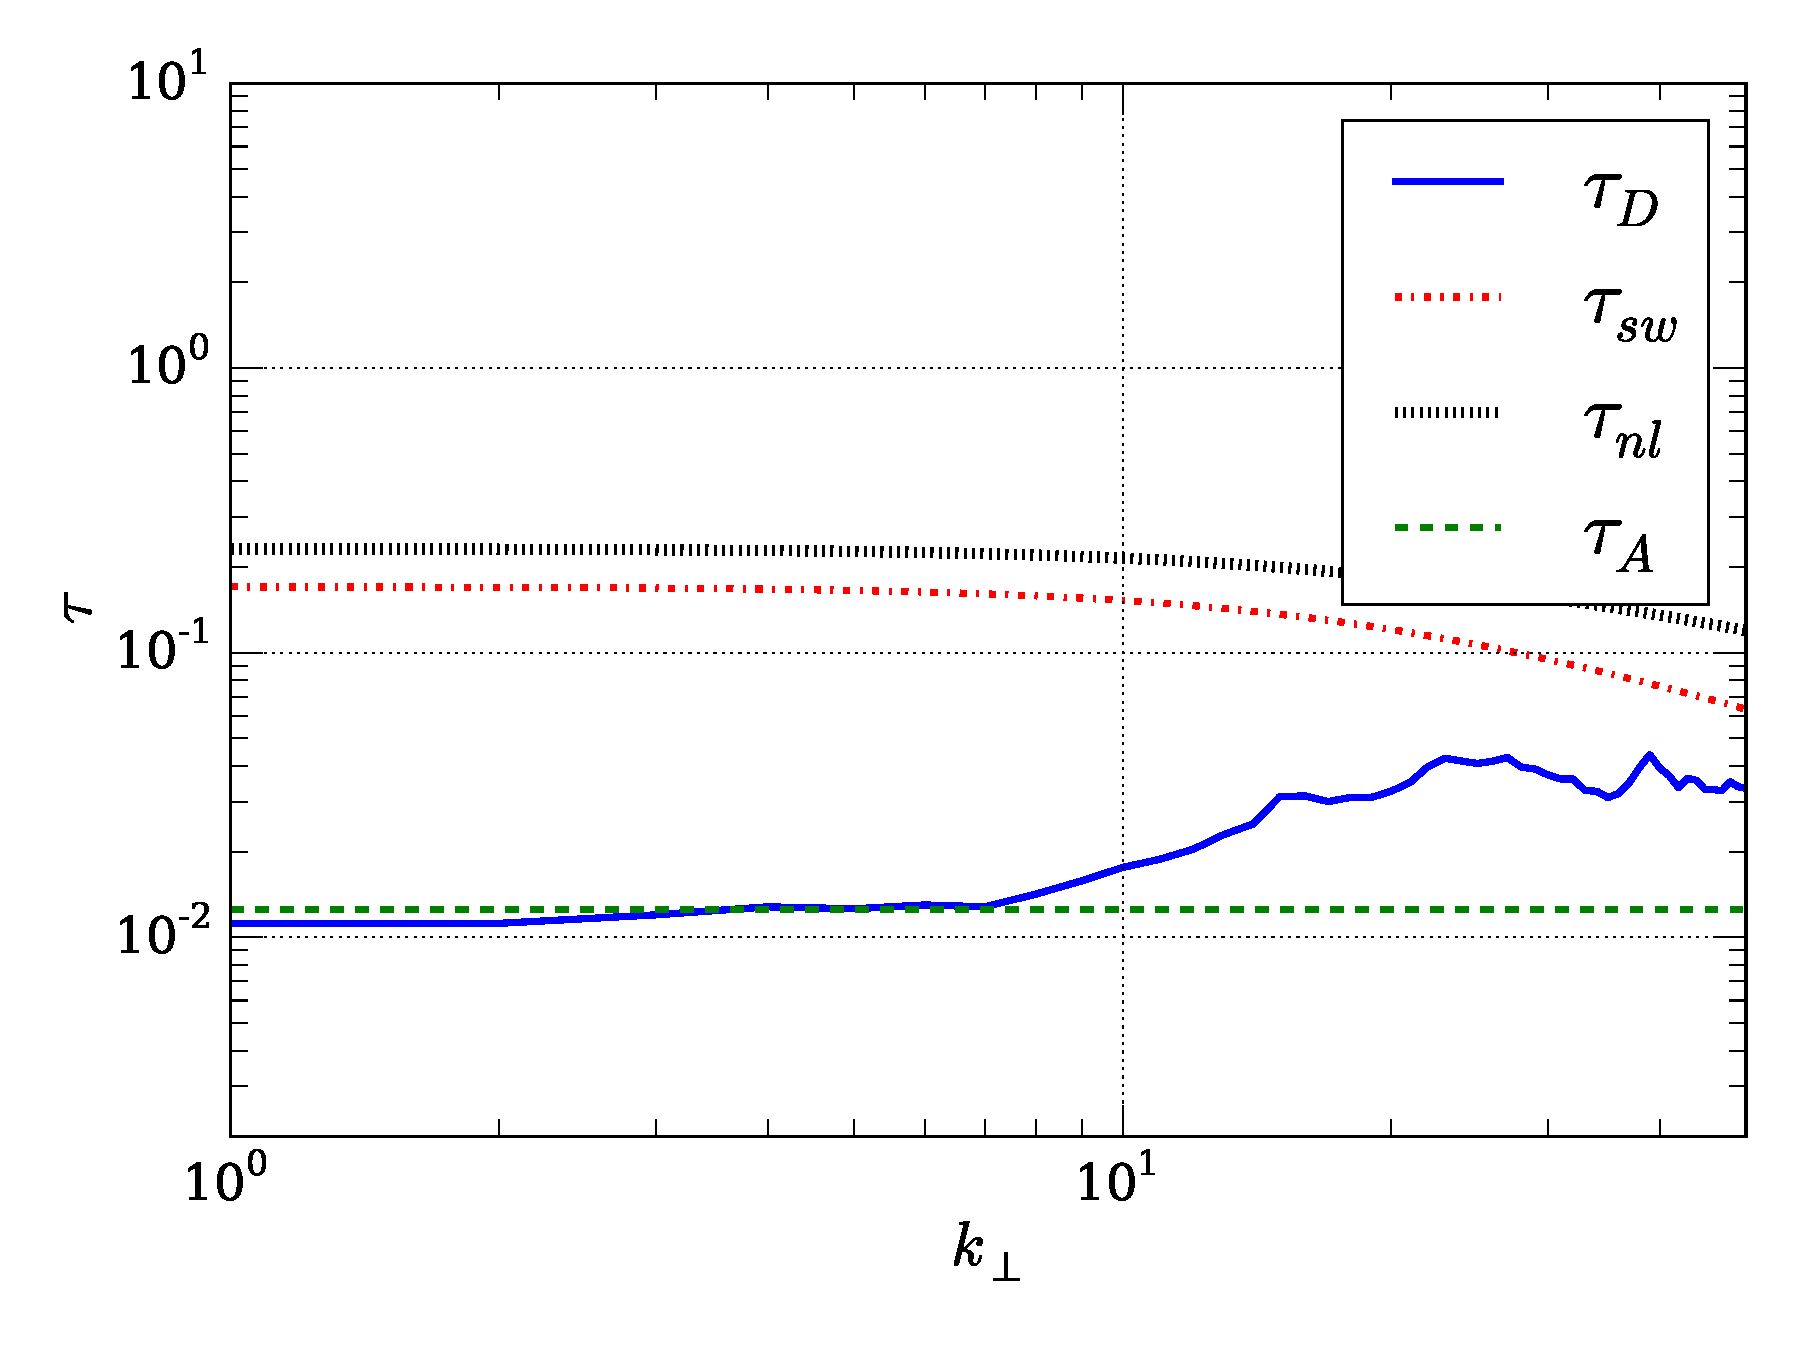
\includegraphics[width=0.7\columnwidth]{figs/fig5_B8_b_kpara_20.pdf}
    \end{center}
  \end{minipage}
}




\frame{\titlepage}

\end{document}
